%-------------- Hardware Description ------------------ %
\section{Implementation}
Overview of the test setup can be seen in FIGURE, Implementation can be divided in three parts
\begin{enumerate}
\item \textbf{Full Spectrum Simulator (FSS):} Which will have the power system model, through which different test conditions will be given
\item \textbf{PMU:} Which will consist of a ADC interfacing board and OMAP-L 137 EVM
\item \textbf{PC:} It will have a Phasor Data Concentrator (PDC), which receives data from the PMU and record it for future analysis.
\end{enumerate}
During the initial phase of the project intention was to use indegenously PMU developed C-DAC but due to the hardware issues and lack of documentation and support, it was decided that a minimalistic PMU will be developed by ourself.

\subsection{Full Spectrum Simulator:}
As per the requirement of the implementation, miniature-Full spectrum Simulator will be used for this purpose. FSS is a card based, multi CPU - parallel processing hardware.It uses TI's MSP430 DSPs as building block. It was developed by IIT Bombay and CDAC for both, offline \& real-time  simulation purposes in Power Electronics and Power Systems.

\begin{figure}[th]
\centering
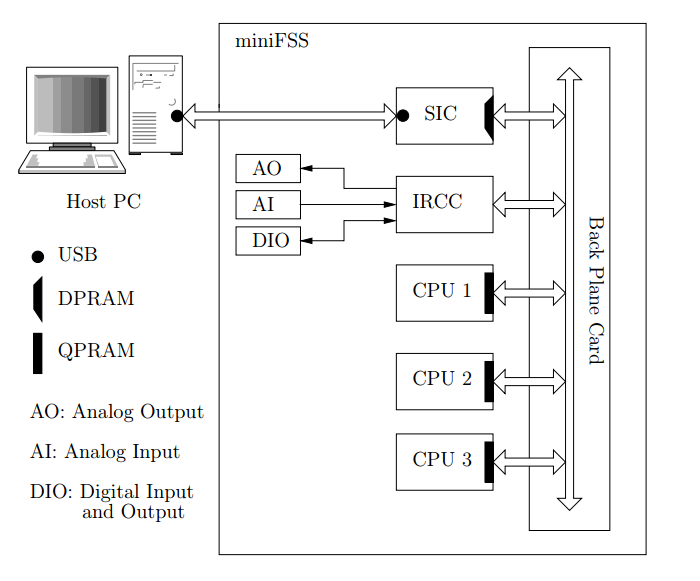
\includegraphics[width=250pt]{fig/fss_arch2.png}
\caption{FSS architecture}
\label{fig:fss_arch}
\end{figure}
As shown in \ref{fig:fss_arch} above it is a card base setup which contains:
\begin{itemize}
\item[-] System Interface Card (SIC)
\item[-] Intra Rack Control Card (IRC Card)
\item[-] Three CPU Cards (CPU 0, CPU 1 and CPU 2), each having 3 digital signal processors on it. So there are total 9 processors allowing for parallel computation.
\item[-] One Analog Output Card (AO Card), having 6 analog output channels (±10 V range).
\item[-]One Analog Input Card (AI Card), having 6 differential analog input channels (±10 V range).
\item[-] One Digital Input/Output Card (DIO Card), having 24 digital inputs and 24 digital outputs (0 - 5 V).
\item[-] One Back Plane PCB.
\end{itemize}


\begin{itemize}
\item \textbf{System Interface Card:} 

It is called SiC, its acts as a communication layer between host PC and the device. Its consists of TUSB chip which connects it to the host PC, a TMS320 to interface SIC with IRC card and a MSP430 to have RS-232 interfacing.
\item \textbf{IRC Card:} IRC is designed as a master control, which eventually control other cards, peripheral communication, timer triggered execution and host pc communication. Further more IRC card handles analog as well as digital input-output also. Apart from that IRC processor also controls the simulation execution using it's timer on the respective CPU card. IRC card has protocal implemented to communicate between CPU cards and SIC so that simulation can be controlled and it's result can be sent to respective peripheral and/or can be downloaded to host PC.

\item \textbf{CPU card:} 

mini-FSS has 3 CPU cards, each having TI's MSP430 DSPs. This card is heart of the FSS. They handle all the mathematical algorithm associated with the simulation. Data flowing from and to the cards are controled by IRC card via \textbf{back plane} PCB.
\end{itemize}

\subsection{PMU}
Omap-L137 EVM is being used as the platform to design a PMU. OMAP-L137 EVM doesnt have Analog to Digital Converter on board hence a interfacing circuit is developed. While designing the ADC board following criteria were kept considered.
\begin{itemize}
\item Good sampling rate: ~200 Samples/Sec
\item No of channels: 3 + 3 = 6 (3 - $\phi$ voltage and current) 
\item Interfacing type: It should be memory addressable and voltage level compatible  to the EVM.
\item Input type: FSS analog output is differential which can be configured as single. their voltage level is $\pm$10V
\end{itemize}

\begin{figure}[ht]
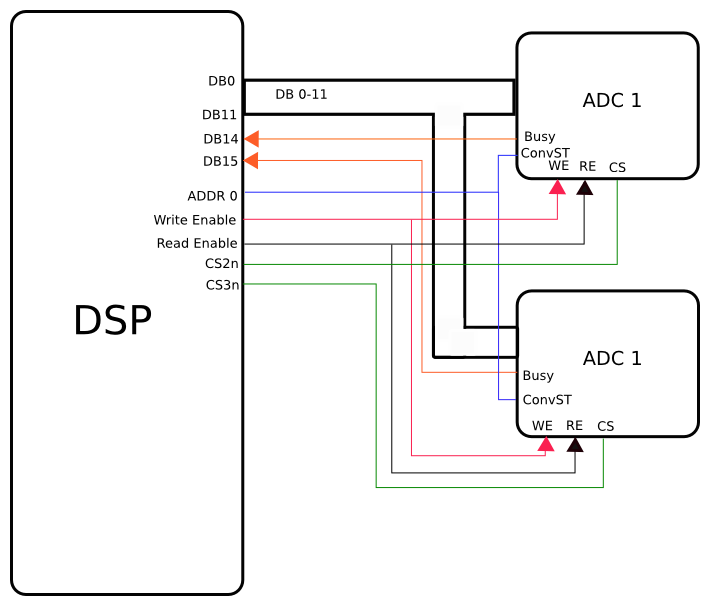
\includegraphics[width=\columnwidth]{fig/ADC_board.png}
\label{fig:adc_board}
\caption{ADC Board block diagram}
\end{figure}
Above Fig:\ref{fig:adc_board}shows the logic of ADC board. Two AD7864-1 are used
